\documentclass[11pt,a4paper]{report}
\usepackage[utf8]{inputenc}
\usepackage{amsmath}
\usepackage{amsfonts}
\usepackage{amssymb}
\usepackage{graphicx}
\usepackage{enumitem}
\usepackage[left=2cm, right=2cm, top=4.5cm, bottom=2cm]{geometry}

\begin{document}
	%Portada
	\begin{titlepage}
		\centering
		{\scshape\LARGE Universidad Nacional Autónoma de México \par}
		\vspace{1cm}
		{\scshape\Large Probabilidad I\par}
		\vspace{1.5cm}
		{\huge\bfseries Tarea Examen\par}
		\vspace{.5cm}

		{\Large\itshape Alan Ernesto Arteaga Vázquez \par}
		 \vspace{.5cm}
		{\Large\itshape Raúl Llamosas Alvarado \par}
		 \vspace{.5cm}
		{\Large\itshape Edgar Quiroz Castañeda \par}
	    \vspace{.5cm}
		{\Large\itshape Jean Paul Ruiz Melo\par}
		\vspace{.5cm}
		{\Large\itshape Sandra Del Mar Soto Corderi \par}

		\vfill
		 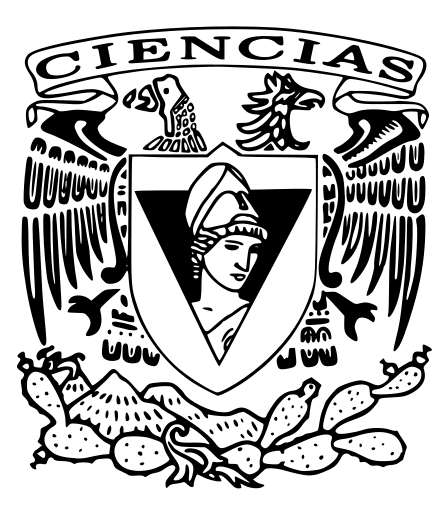
\includegraphics[width=0.3\textwidth]{escudo.png}
		\vfill

		{\large Lunes 3 de Diciembre del 2018 \par}
	\end{titlepage}

	\pagebreak
	\setlength{\voffset}{-0.75in}
	\setlength{\headsep}{5pt}

	%Ejericios
	\begin{enumerate}
		%1
		\item{

		\newcommand{\Size}{1cm}
        \def\NumOfColumns{5}
        \def\Sequence{1/A, 2/B, 3/C, 4/D, 5/E}
        \tikzset{Square/.style={
            inner sep=0pt,
            text width=\Size,
            minimum size=\Size,
            draw=black,
            fill=white,
            align=center
            }
        }
        \newcommand{\NodeAA}{$\frac{y}{x}$}\newcommand{\NodeAB}{1}\newcommand{\NodeAC}{2}%
        \newcommand{\NodeAD}{3}\newcommand{\NodeAE}{4}%

        \newcommand{\NodeBA}{1}\newcommand{\NodeBB}{$(1,1)$}\newcommand{\NodeBC}{$(1,2)$}%
        \newcommand{\NodeBD}{$(1,3)$}\newcommand{\NodeBE}{$(1,4)$}%

        \newcommand{\NodeCA}{2}\newcommand{\NodeCB}{$(1,2)$}\newcommand{\NodeCC}{$(2,2)$}%
        \newcommand{\NodeCD}{$(2,3)$}\newcommand{\NodeCE}{$(2,4)$}%

        \newcommand{\NodeDA}{3}\newcommand{\NodeDB}{$(1,3)$}\newcommand{\NodeDC}{$(2,3)$}%
        \newcommand{\NodeDD}{$(3,3)$}\newcommand{\NodeDE}{$(3,4)$}%

        \newcommand{\NodeEA}{4}\newcommand{\NodeEB}{$(1,4)$}\newcommand{\NodeEC}{$(2,4)$}%
        \newcommand{\NodeED}{$(3,4)$}\newcommand{\NodeEE}{$(4,4)$}%

        \newcommand{\NodeFF}{$\frac{y}{x}$}\newcommand{\NodeFG}{1}\newcommand{\NodeFH}{2}%
        \newcommand{\NodeFI}{3}\newcommand{\NodeFJ}{4}\newcommand{\NodeFK}{$f_X(x)$}%

        \newcommand{\NodeGF}{1}\newcommand{\NodeGG}{$\frac{1}{16}$}\newcommand{\NodeGH}
        {$\frac{2}{16}$}\newcommand{\NodeGI}{$\frac{2}{16}$}\newcommand{\NodeGJ}
        {$\frac{2}{16}$} \newcommand{\NodeGK}{$\frac{7}{16}$}%

        \newcommand{\NodeHF}{2}\newcommand{\NodeHG}{0}\newcommand{\NodeHH}{$\frac{1}{16}$}%
        \newcommand{\NodeHI}{$\frac{2}{16}$}\newcommand{\NodeHJ}{$\frac{2}{16}$}%
        \newcommand{\NodeHK}{$\frac{5}{16}$}%

        \newcommand{\NodeIF}{3}\newcommand{\NodeIG}{0}\newcommand{\NodeIH}{0}%
        \newcommand{\NodeII}{$\frac{1}{16}$}\newcommand{\NodeIJ}{$\frac{2}{16}$}%
        \newcommand{\NodeIK}{$\frac{3}{16}$}%

        \newcommand{\NodeJF}{4}\newcommand{\NodeJG}{0}\newcommand{\NodeJH}{0}%
        \newcommand{\NodeJI}{0} \newcommand{\NodeJJ}{$\frac{1}{16}$}%
        \newcommand{\NodeJK}{$\frac{1}{16}$}%

        \newcommand{\NodeKF}{$f_Y(y)$}\newcommand{\NodeKG}{$\frac{1}{16}$}%
        \newcommand{\NodeKH}{$\frac{3}{16}$} \newcommand{\NodeKI}{$\frac{5}{16}$}%
        \newcommand{\NodeKJ}{$\frac{7}{16}$}%

		Considere el experimento de lanzar dos tetraedros cuyos lados están numerados del 1 al 4. Sean $Y_{1},Y_{2}$ los números más pequeño y más grande obtenidos en las caras superiores respectivamente.\\
		Tenemos lo siguiente:
		\\
    	\centerline{
    	\begin{tikzpicture}[draw=black, ultra thick, x=\Size,y=\Size]
        \foreach \col/\colLetter in \Sequence {%
            \foreach \row/\rowLetter in \Sequence{%
                \pgfmathtruncatemacro{\value}{\col+\NumOfColumns*(\row-1)}
                \def\NodeText{\expandafter\csname Node\rowLetter\colLetter\endcsname}
                \node [Square] at ($(\col,-\row)-(0.5,0.5)$) {\NodeText};
                }
            }
        \end{tikzpicture}
        }

        \def\Sequence{1/F, 2/G, 3/H, 4/I, 5/J, 6/K}


		    \begin{enumerate}
		        %(a)
		        \item {Encuentre la función de densidad conjunta de $Y_{1},Y_{2}$}\\
		        De esto se tiene:\\
		      \centerline{
    	            \begin{tikzpicture}[draw=black, ultra thick, x=\Size,y=\Size]
                         \foreach \col/\colLetter in \Sequence {%
                                \foreach \row/\rowLetter in \Sequence{%
                                    \pgfmathtruncatemacro{\value}{\col+6*(\row-1)}
                                    \def\NodeText{\expandafter\csname Node\rowLetter\colLetter\endcsname}
                                    \node [Square] at ($(\col,-\row)-(0.5,0.5)$) {\NodeText};
                                 }
                        }
                 \end{tikzpicture}
                }


		        %(b)
		        \item{Obtenga la densidad condicional de $Y_{2}$ dado $Y_{1}$ para cada uno de los posibles valores de $Y_{1}$}
		        \[ f(1|X) =\frac{P(X = x, Y = 1)}{P(X = x)} =
		        \frac{\frac{1}{16}}{\frac{7}{16}} +
		        \frac{\frac{2}{16}}{\frac{7}{16}} +
		        \frac{\frac{2}{16}}{\frac{7}{16}} +
		        \frac{\frac{2}{16}}{\frac{7}{16}} =
		        .14 + .28 + .28 + .28\]
		        \[ f(2|X) =\frac{P(X = x, Y = 2)}{P(X = x)} =
		        \frac{0}{\frac{5}{16}} +
		        \frac{\frac{1}{16}}{\frac{5}{16}} +
		        \frac{\frac{2}{16}}{\frac{5}{16}} +
		        \frac{\frac{2}{16}}{\frac{5}{16}} =
		        .2 + .4 + .4\]
		        \[ f(3|X) =\frac{P(X = x, Y = 3)}{P(X = x)} =
		        \frac{0}{\frac{3}{16}} +
		        \frac{0}{\frac{3}{16}} +
		        \frac{\frac{1}{16}}{\frac{3}{16}} +
		        \frac{\frac{2}{16}}{\frac{3}{16}} =
		        .33 + .66\]
		        \[ f(4|X) =\frac{P(X = x, Y = 4)}{P(X = x)} =
		        \frac{0}{\frac{1}{16}} +
		        \frac{0}{\frac{1}{16}} +
		        \frac{0}{\frac{1}{16}} +
		        \frac{\frac{1}{16}}{\frac{1}{16}} = 1\]
		        %(c)
		        \item{Encuentre $E(Y_{1}Y_{2}),E(Y_{1}),E(Y_{2})$}\\
		        \[E(Y_{1}Y_{2}) = E(XY) =
		        \frac{1}{16} + 2\frac{2}{16} +3\frac{2}{16} +4\frac{2}{16} +
		       0 + (2\times2)\frac{1}{16} + (2\times3)\frac{2}{16} + (2\times4)\frac{2}{16} +\]
		        \[0 + 0 + (3\times3)\frac{1}{16} + (3\times4)\frac{2}{16} + 0 + 0 + 0 + (4\times4)\frac{1}{16}\]
		        \[= \frac{1}{16} + \frac{4}{16} + \frac{6}{16} + \frac{8}{16} + \frac{4}{16} + \frac{12}{16} + \frac{16}{16} +
			\frac{9}{16} + \frac{24}{16} + \frac{16}{16} = \frac{84}{16} = 5.25\]
		        \[E(Y_1) = E(X) = \frac{7}{16} + 2(\frac{5}{16}) + 3(\frac{3}{16}) + 4(\frac{1}{16}) = 1.875\]
		        \[E(Y_2) = E(Y) = \frac{1}{16} + 2(\frac{3}{16}) + 3(\frac{5}{16}) + 4(\frac{7}{16}) = 3.125\]

		        %(d)
		        \item{¿Son $Y_{1} $ y $Y_{2}$ independientes?}\\
		        Tenemos que para que sea independiente se debe cumplir que:
		        \[f_{X,Y}(x,y) = f_X(x)f_Y(y)\]
		        Entonces si $x=1,y=1$, ya vimos que $f_{X,Y}(1,1) = \frac{1}{16}$ , $f_X(1) = \frac{7}{16}$ y $f_Y(1) =
			\frac{1}{16}$, entonces:
		         \[f_{X,Y}(1,1) = \frac{1}{16} \neq \frac{7}{256} = \frac{7}{16}\frac{1}{16} = f_X(1)f_Y(1)\]
		         Por lo tanto $Y_1$ y $Y_2$ no son independientes.

		    \end{enumerate}
		}

		%2
		\item{
		Suponga que X es una variable aleatoria con distribución $Bin(100,\frac{1}{5})$. Utilizando el teoerema de DeMoivre-
		Laplace, calcular $P(15\leq X \leq 25)$. \\
		Tenemos que DeMoivre-Laplace dice:
		\[X-Bin(n,p) =\frac{x-np}{\sqrt{np(1-p)}} = z = \frac{x - 100(\frac{1}{5})}{\sqrt{100(\frac{1}{5})(\frac{4}{5})}} =
		\frac{x - 20}{4}\]
		Para X-N(0,1), entonces:
		\[P(15 \leq X \leq 25) = \phi(\frac{25 - 20}{4}) - \phi(\frac{15 - 20}{4})  =
		\phi(\frac{5}{4}) - \phi(\frac{-5}{4}) = \phi(\frac{5}{4}) - (1 - \phi(\frac{5}{4}))\]
		\[\phi(1.25) - 1 + \phi(1.25) = 2( ) - 1 = 2(.8944) - 1 = 1.7888 - 1 = .7888\]
		}

		%3
		\item{
            En una tarde soleada, Augusto lanza dos dados 2160 veces (él casi no tiene nada que hacer). Sea X el número de veces que 2 aparece en alguna de las caras. Encontrar la probabilidad de que X sea menor a 55. \\            Esto describe una Binomial con parámetros 2160 y $p=\frac{11}{36}$ entonces se sigue que $$P(X\leq 54)= \sum_{i=0}^{54}\binom{2160}{i}(\frac{11}{36})^i(\frac{25}{36})^{2160-i}$$
            Pero tomando en cuenta que la binomial son 2160 eventos bernoulli independientes se sigue que $\lbrace X_{i} \rbrace _{i=1}^{2160}$ son todos eventos bernoulli de forma que su esperanza y varianza son $Var(X)=\frac{(11)(25)}{36^2}$ y $E(X)=\frac{11}{36}$ y el teorema de limite central nos dice que 
            $$P\lbrace  X_{1}+...X_{2160}\leq 54 \rbrace = P\lbrace \frac{\sum_{i=1}^{2160}X_{i} -2160(\frac{11}{36})}{\sqrt{2160(\frac{11(25)}{36^2})}}\leq \frac{54-2160(\frac{11}{36})}{\sqrt{2160(\frac{11(25)}{36^2})}}\rbrace \rightarrow \Phi(\frac{54-2160(\frac{11}{36})}{\sqrt{2160(\frac{11(25)}{36^2})}})$$
            Y como
            $$\frac{54-2160(\frac{11}{36})}{\sqrt{2160(\frac{11(25)}{36^2})}}=-28.306$$
            Y esa probabilidad tiende a cero. Entonces $$P(X<55)\approx 0$$
		}

		%4
		\item{
			Sean $X_{1},...,X_{n}$ variables aleatorias independientes. Use la función generadora de momentos para encontrar la distribución de $\sum_{i=1}^{n}X_{i}$ en los siguientes casos:\\
			\begin{enumerate}
			    %(a)
			    \item {Si $\forall i \ \in \lbrace 1,..,n \rbrace \ X_{i} \sim Gamma(r,\lambda)$}
	        Tenemos que si $Z=\sum_{i=1}^{n}X_{i}$ entonces la función generadora de momentos de Z denotada por $Mg_{Z}(t)$ está dada por:
	        $$Mg_{Z}(t)=\prod_{i=1}^{n} Mg_{X_{i}}(t)$$ pero como $\forall \ i \ Mg_{X_{i}}(t)=(\frac{\lambda}{\lambda-t})^{r}$ entonces
	        $$\prod_{i=1}^{n}(\frac{\lambda}{\lambda-t})^{r}=(\frac{\lambda}{\lambda-t})^{\sum_{i=1}^{n}r}=(\frac{\lambda}{\lambda-t})^{nr}$$
	        Pero si esa es la función generadora de Z entonces se tiene que $$Z \sim Gamma(nr,\lambda)_{\blacksquare}$$
	     %(b)
			    \item{Si $\forall i \ \in \lbrace 1,..,n \rbrace \ X_{i} \sim Gamma(r_{i},\lambda)$ } \\
			    Análogamente como en el anterior, usamos la generadora de momentos y tenemos que
			    $$Mg_{Z}(t)=\prod_{i=1}^{n}Mg_{X_{i}}(t)=\prod_{i=1}^{n}(\frac{\lambda}{\lambda-t})^{r_{i}}=(\frac{\lambda}{\lambda-t})^{\sum_{i=1}^{n}r_{i}}$$
			    Entonces se sigue que $$Z\sim Gamma(\sum_{i=1}^{n}r_{i},\lambda)_{\blacksquare}$$
			   
         %(c)
                \item{Si $\forall i \ \in \lbrace 1,..,n \rbrace \ X_{i} \sim exp(\lambda)$ }\\
                La función generadora de $Z=\sum_{i=1}^{n}X_{i}$, donde cada $X_{i}$ tiene generadora de momentos $Mg_{X_{i}}(t)=\frac{\lambda}{\lambda-t}$ es 
                $$Mg_{Z}(t)=\prod_{i=1}^{n}(\frac{\lambda}{\lambda-t})=(\frac{\lambda}{\lambda-t})^{n}$$
                Pero esa es la generadora de momentos de una Gamma con parametro n, $\lambda$ entonces:
                $$Z\sim Gamma(n,\lambda)_{\blacksquare}$$
                %(d)
                \item{Si $\forall i \ \in \lbrace 1,..,n \rbrace \ X_{i} \sim Geo(p)$ }\\
                La función generadora de momentos de una variable aleatoria $Z=\sum_{i=1}^{n}X_{i}$ donde cada $X_{i}$ tiene generadora de momentos $Mg_{X_{i}}(t)=\frac{p}{1-(1-p)e^t}$ está dada por
                $$Mg_{Z}(t)=\prod_{i=1}^{n}(\frac{p}{1-(1-p)e^t})=(\frac{p}{1-(1-p)e^t})^n$$ Lo cual es idéntica a una distribución binomial negativa con parámetro n,p.Entonces 
                $$Z\sim BinNeg(n,p)_{\blacksquare}$$
                %(e)
                \item{Si $\forall i \ \in \lbrace 1,..,n \rbrace \ X_{i} \sim BinNeg(r,p)$ }\\
                La función generadora de momentos de una variable aleatoria $Z=\sum_{i=1}^{n}X_{i}$ donde cada $X_{i}$ tiene generadora de momentos $Mg_{X_{i}}(t)=(\frac{p}{1-(1-p)e^t})^r$ está dada por:
                $$Mg_{Z}(t)=\prod_{i=1}^{n}(\frac{p}{1-(1-p)e^t})^r=(\frac{p}{1-(1-p)e^t})^{\sum_{i=1}^{n}r}=(\frac{p}{1-(1-p)e^t})^{nr}$$
                Entonces se sigue que 
                $$Z \sim BinNeg(nr,p)_{\blacksquare}$$
                %(f)
                \item{Si $\forall i \ \in \lbrace 1,..,n \rbrace \ X_{i} \sim BinNeg(r_{i},p)$ }\\
                La función generadora de momentos de una variable aleatoria $Z=\sum_{i=1}^{n}X_{i}$ donde cada $X_{i}$ tiene generadora de momentos $Mg_{X_{i}}(t)=(\frac{p}{1-(1-p)e^t})^{r_{i}}$ está dada por:
                $$Mg_{Z}(t)=\prod_{i=1}^{n}(\frac{p}{1-(1-p)e^t})^{r_{i}}=(\frac{p}{1-(1-p)e^t})^{\sum_{i=1}^{n}r_{i}}$$ Entonces se sigue que 
                $$Z\sim BinNeg(\sum_{i=1}^{n}r_{i},p)_{\blacksquare}$$
                %(g)
                \item{Si $\forall i \ \in \lbrace 1,..,n \rbrace \ X_{i} \sim Poisson(\lambda)$ }\\
                La función generadora de momentos de una variable aleatoria $Z=\sum_{i=1}^{n}X_{i}$ donde cada $X_{i}$ tiene generadora de momentos $Mg_{X_{i}}(t)=e^{\lambda(e^t-1)}$ está dada por:
                $$Mg_{Z}(t)=\prod_{i=1}^{n}(e^{\lambda(e^t-1)})=(e^{\lambda(e^t-1)})^n=(e^{n\lambda (e^t-1)})$$
                Entonces se sigue que 
                $$Z\sim Poisson(n\lambda)_{\blacksquare}$$
                
                %(h)
                \item{Si $\forall i \ \in \lbrace 1,..,n \rbrace \ X_{i} \sim Bin(n,p)$}\\
                La función generadora de momentos de una variable aleatoria $Z=\sum_{i=1}^{n}X_{i}$ donde cada $X_{i}$ tiene una generadora de momentos $Mg_{X_{i}}(t)=(e^t p+(1-p))^n$ está dada por:
                $$Mg_{Z}(t)=\prod_{i=1}^n (e^t p+(1-p))^n=(e^t p+(1-p))^{n^2}$$
                Entonces se sigue que 
                $$Z \sim Bin(n^2,p)_{\blacksquare}$$
                \textbf{Nota:} La notación del ejercicio infiere que el número de variables aleatorias coincide con el parámetro n. De ser éste el caso entonces distribuye como mencionamos arriba. Si ésta no era la intención entonces distribuye $Bin(n(k),p)$ donde k es el parámetro con el cual cada $X_{i}$ distribuye de forma binomial.
        
                %(i)
                \item{Si $\forall i \ \in \lbrace 1,..,n \rbrace \ X_{i} \sim Bin(n_{i},p)$ } \\
                La función generadora de momentos de una variable aleatoria $Z=\sum_{i=1}^{n}X_{i}$ donde cada $X_{i}$ tiene una generadora de momentos $Mg_{X_{i}}(t)=(e^t p+(1-p))^{n_{i}}$ está dada por:
                $$Mg_{Z}(t)=\prod_{i=1}^{n}(e^t p+(1-p))^{n_{i}}=(e^t p+(1-p))^{\sum_{i=1}^{n}n_{i}}$$
                Entonces se sigue que:
                $$Z\sim Bin(\sum_{i=1}^{n}n_{i},p)_{\blacksquare}$$
                %(j)
                \item{Si $\forall i \ \in \lbrace 1,..,n \rbrace \ X_{i} \sim N(\mu,\sigma_{i}^2)$ }\\
                La función generadora de momentos de una variable aleatoria $Z=\sum_{i=1}^{n}X_{i}$ donde cada $X_{i}$ tiene una generadora de momentos $Mg_{X_{i}}(t)=e^{t\mu +\frac{t^2 \sigma_{i} ^2}{2}}$ está dada por:
                $$Mg_{Z}(t)=\prod_{i=1}^{n} e^{t\mu +\frac{t^2 \sigma_{i} ^2}{2}}=e^{\sum_{i=1}^{n}t\mu + \frac{t^2 \sigma_{i} ^2}{2}}=e^{t\sum_{i=1}^{n}\mu+\frac{t^2}{2}\sum_{i=1}^{n}\sigma_{i} ^2}$$
                Entonces se sigue que 
                $$Z\sim N(\sum_{i=1}^{n}\mu,\sum_{i=1}^{n} \sigma_{i}^2)_{\blacksquare} $$
                
			\end{enumerate} 
		}

		%5
		\item{
		Sea $S_{n}$ el número de éxitos en n ensayos Bernouilli independientes.
        Demuestre que
        $$P(|\frac{S_{n}}{n}-p|\geq \epsilon)\leq \frac{1}{4n\epsilon^2}$$
        Digamos que $S_{n} = \sum_{i=1}^{n}{X_{i}}$
		Veamos cual es la esperanza y la varianza de $\frac{S_{n}}{n}$.
        \[E(\frac{S_{n}}{n}) = \frac{1}{n}E(S_{n})
        = \frac{1}{n}\sum_{i=1}^{n}{E(X_{i})} = \frac{1}{n}\sum_{i=1}^{n}{p_{i}}\]
        \[Var(\frac{S_{n}}{n}) = \frac{1}{n^2}E(S_{n})
        = \frac{1}{n^2}\sum_{i=1}^{n}{Var(X_{i})} =
        \frac{1}{n^2}\sum_{i=1}^{n}{p_{i}(p_{i}-1)}\]
        Si tenemos que los ensayos Bernoulli son identicamente distribuidos,
        es decir que $p_i = p$ tenemos que
        \[E(\frac{S_{n}}{n}) = \frac{1}{n}\sum_{i=1}^{n}{p} = p\]
        \[Var(\frac{S_{n}}{n}) = \frac{1}{n^2}\sum_{i=1}^{n}{p(1-p)}
        =\frac{p(1-p)}{n}\]
        Entonces, por la desigualdad de Chevyshev
        \begin{align*}
            P(|\frac{S_{n}}{n} - E(\frac{S_{n}}{n})| \geq \epsilon) &\leq
            \frac{Var(\frac{S_{n}}{n})}{\epsilon^2}\\
            P(|\frac{S_{n}}{n} - p| \geq \epsilon) &\leq
            \frac{\frac{p(1-p)}{n}}{\epsilon^2} \\
            &=\frac{p(1-p)}{n\epsilon^2}
        \end{align*}
        Ahora hay que ver cual es el valor máximo de $p(1-p) = p - p^2$.
        \begin{align*}
            \frac{d(p - p^2)}{dp} &= 1 - 2p = 0 \\
            &\implies p = \frac{1}{2}\\
            \frac{d(1 - 2p)}{dp} &= -2
        \end{align*}
        Por lo que $p(1-p)$ alcanza un máximo en $p = \frac{1}{2}$.
        Entonces, el máximo posible valor de $p(1-p)$ es
        \[\frac{1}{2}(1-\frac{1}{2}) = \frac{1}{2}\cdot \frac{1}{2} = \frac{1}{4}\]
        Por lo que, para cualquier valor de $p$, tenemos que
        $p(1-p)\leq \frac{1}{4}$.
        Entonces, en particular
        \[\frac{p(1-p)}{n\epsilon^2} \leq \frac{\frac{1}{4}}{n\epsilon^2}
        = \frac{1}{4n\epsilon^2}\]
        Por lo que se tiene la desigualdad
        \[P(|\frac{S_{n}}{n}-p|\geq \epsilon)\leq \frac{1}{4n\epsilon^2}\]
		}

		%6
		\item{
		Sea S el número de águilas en 1,000,000 lanzamientos de una moneda
        honesta. Use (a) la desigualdad de Chebyshev y (b) el Teorema del
        Límite Central para estimar la probabilidad de que S esté entre 499,500
        y 500,500.\\
        Primero veamos como se comporta $S$.\\
        $X$ es la cantidad de águilas en un lanzamiento de esa moneda, entonces
        $X \sim Bernoulli(\frac{1}{2})$.\\
        Entonces $E(X) = \frac{1}{2}$ y $Var(X) = \frac{1}{4}$
        Como $S$ se obtiene realizando y sumando 1,000,000 veces $X$, entonces,
        \begin{align*}
            S &= \sum_{i=1}^{1,000,000}{X}\\
            E(S) &= \sum_{i=1}^{1,000,000}{E(X)}
            = \sum_{i=1}^{1,000,000}{\frac{1}{2}}
            =500,000\\
            Var(S)&= \sum_{i=1}^{1,000,000}{Var(X)}
            = \sum_{i=1}^{1,000,000}{\frac{1}{4}}
            = 250,000
        \end{align*}
        Pues el lanzamiento de moneda es independiente en cada ocasión.\\
        Ahora veamos los incisos
        \begin{enumerate}
            %a
            \item {
            \[P(499,500\leq S\leq
             500,500)=P(|S-500,000)|\leq500)=1-P(|S-500,000)|>500)\]
            Luego, por la desigualdad de Chebyshev, tenemos que
            \[P(|S-500,000)|> 500)<\frac{500^2}{250,000} = 1\]
            Entonces
            \[P(499,500\leq S\leq 500,500)=1-P(|S-500,000)|>500)>1 - 1 = 0\]
            }

            %b
            \item {
            Por el TLC tenem que si $X_i, \dots, X_n$ son independientes e
            indenticamente distribuidas.
            \[P \Big\{ \frac{X_1 + \dots + X_n - nE(X_i)}
            {\sqrt{nVar(X_i)}} \leq k \Big\}  \to \Phi(k)\]
            }
            Cuando $n \to \infty$.\\
            En este caso, tenemos que $S$ es la suma de variables
            aleatorias independientes e indenticamente distribuidas y
            $n = 1,000,000$.
            \begin{align*}
                P \Big\{ \frac{S - \frac{1,000,000}{2}}
                {\sqrt{\frac{1,000,000}{4}}} \leq k \Big\}
                &= P \Big\{ \frac{S - 500,000}
                {500} \leq k \Big\}
                = P \Big\{ \frac{S}{500} - 1,000
                 \leq k \Big\} \\
                &= P \Big\{S
                 \leq 500(k+1000) \Big\} \to \Phi(k) \\
            \end{align*}
            Por otra, tenemos que
            \[P(499,500\leq S\leq 500,500) = P(S \leq 500,500) - P(S \leq 499,500)
            +P(S = 499,500)\]
            Pero como $S$ se distribute continua, pues $n$ es grande,
            $P(S = 499,500) \approx 0$.\\
            Luego,
            \begin{align*}
                500,500 &= 500(k_1+1000) \implies 1,001 = k_1 + 1000 \implies k_1 = 1 \\
                499,500 &= 500(k_2+1000) \implies 999 = k_2 + 1000 \implies k_2 = -1
            \end{align*}
            Por lo que
            \begin{align*}
                P(499,500\leq S\leq 500,500) &\approx
                P(S \leq 500,500) - P(S \leq 499,500)\\
                &= P(S \leq 500(1+1000)) - P(S \leq 500(-1+1000)) \\
                &\approx \Phi(1) - \Phi(-1) = \Phi(1) - (1 - \Phi(1)) \\
                &= 0.5 - 1 + 0.5 = 0
            \end{align*}
        \end{enumerate}
		}

		%7
		\item{
		
          Si $X \sim Gamma(n,1)$ aproximadamente que tan grande debe ser n para que 
          $$P[|\frac{X}{n}-1| > 0.01] < 0.01$$
          
          Definamos $X_{i} \sim Exp(1)$, como hemos visto en clase, Gamma es una generalización de Exponencial, entonces podemos decir que:
          
          $X = \sum_{i=1}^{n} X_{i}$,
          
          Así podemos ver que:
          
           $P[|\frac{X}{n}-1| > 0.01] < 0.01 = P[|\frac{\sum_{i=1}^{n} X_{i}}{n}-1| > 0.01] < 0.01$\\
           
           $= P[|\frac{\sum_{i=1}^{n} X_{i} -n}{n}| > 0.01] < 0.01$\\
           
           Sabemos que el Teorema del Limite Central dice que:
				
 				z = $\frac{\sum_{i=1}^{n} X_{i} - \mu n }{\sigma \sqrt{n}}  \xrightarrow{n \to \infty}  z \sim N(0,1)$\\
			            
          Vemos que la exponencial y varianza valen 1, es decir, $\mu = 1$ y $\sigma = 1$, así que para que nuestra expresión sea igual al teorema del límite central, necesitamos una $\sqrt{n}$ en el denominador, esto lo podemos conseguir multiplicando por $\sqrt{n}$ los dos lados de la desigualdad, esto no afecta, ya que la raíz cuadrada respeta el valor absoluto, entonces tenemos:
          
          $= P[|\frac{\sum_{i=1}^{n} X_{i} -n}{\sqrt{n}}| > 0.01\sqrt{n}] < 0.01$
          
          Vemos que es igual a la definición del Teorema del Límite Central y aplicandolo tenemos que cuando $n \to \infty$:
          
          $P( |z| > 0.01\sqrt{n} ) < 0.01$
          
          $ = (1 - P(z \leq 0.01\sqrt{n})) < 0.01$
          
          $ = (1 - \phi(0.01\sqrt{n})) < 0.01$
          
          $ = - \phi(0.01\sqrt{n}) < 0.01 - 1$
          
         $ = \phi(0.01\sqrt{n}) > 0.99$
          
        Revisando la tabla de distribución de la normal, podemos observar que el primer valor donde $\phi$ es mayor a 0.99 es 2.33, entonces:
        
        $\phi(2.33) > 0.99$  y  $\phi(0.01\sqrt{n}) > 0.99$\\
        
        De ahí, 
        
        $0.01\sqrt{n} = 2.33$
        
        $\sqrt{n} = \frac{2.33}{0.01}$
        
        $n = (\frac{2.33}{0.01}) ^ 2 = 54289$\\
        
        Por lo tanto n debe ser al menos 54289 para que $P[|\frac{X}{n}-1| > 0.01] < 0.01$\\

		}

		%8
		\item{
			Sean $X_{1},...,X_{20}$ variables aleatorias independientes tales que $\forall i \ \in \lbrace 1,...,20 \rbrace \ X_{i} \sim Poisson(\lambda) $ con media 1.\\
			\begin{enumerate}
			    %(a)
          
			    \item{Utilice la desigualdad de Markov para obtener una cota para $P[\sum_{i=1}^{20}X_{i}>15]$} 
			    
			    Sabemos que la desigualdad de Markov dice que:
			    
			    $P(g(x) \geq k) \leq \frac{E(g(x))}{k}$\\
			    
			    Ya que la esperanza de cada $X_{i}$ es 1, la esperanza de la suma, es 20.
		    
			    Sustituimos en la desigualdad y tenemos que:\\
			    
			    $P(\sum_{i=1}^{20}X_{i}>15) < \frac{E(\sum_{i=1}^{20}X_{i})}{15} = \frac{20}{15}$\\
			    
			    Otra forma de ver el problema es:
			    
			    $P(\sum_{i=1}^{20}X_{i}\geq 16) \leq \frac{E(\sum_{i=1}^{20}X_{i})}{16} = \frac{20}{16}$\\
			        
			 
			    %(b)
			    \item{Utilice el Teorema del Limite Central para aproximar $P[\sum_{i=1}^{20}X_{i}>15]$}
			    
				Sabemos que el Teorema del Limite Central dice que:
				
 				z = $\frac{\sum_{i=1}^{n} X_{i} - \mu n }{\sigma \sqrt{n}}  \xrightarrow{n \to \infty}  z \sim N(0,1)$\\
			    
				Ya que la esperanza de la suma es 20, al ser distribución poisson, sabemos que la varianza es igual a la esperanza, entonces la esperanza de la suma también es 20, es decir $\mu = 20$ y $\sigma = \sqrt{20}$, sustituimos en el teorema y tenemos:
				
				z = $\frac{\sum_{i=1}^{20} X_{i} - 20n }{\sqrt{20n}}  \xrightarrow{n \to \infty}  z \sim N(0,1)$\\
				
				Entonces tenemos que:
				
				$P(z > \frac{15 - 20}{\sqrt{20}}) = 1 - P(z \leq \frac{15 - 20}{\sqrt{20}}) = 1 - \phi (\frac{15 - 20}{\sqrt{20}}) = 1 - \phi(-\frac{\sqrt{5}}{2})$
				$= 1 - (1 - \phi (\frac{\sqrt{5}}{2})) = \phi(\frac{\sqrt{5}}{2})$
				$\approx \phi(1.11) = 0.8665$\\
				
				Por lo tanto:
				
				$P[\sum_{i=1}^{20}X_{i}>15] \approx 0.8665$\\
			\end{enumerate}
		}

		%9
		\item{
	    Sea $\lbrace X_{i} \rbrace _{i=1}^{\infty}$ una sucesión de variables aleatorias independientes. Suponga que $E(X_{i})=0$ y $Var(X_{i})=\sigma_{i}^{2}$ y suponga también que:
	            $$\lim_{n \rightarrow \infty}\sum_{i=1}^{n}\frac{\sigma_{i}^{2}}{n^2}=0$$
	   Demuestre que para cualquier $\epsilon >0$
	                $$P(\frac{|\sum_{i=1}^{n}X_{i}|}{n}>\epsilon)\rightarrow 0$$
	   Cuando $n\rightarrow \infty$.\\
	   Use lo anterior para probar que si $\lbrace Y_{i} \rbrace_{i=1}^{\infty}$ son variables aleatorias independientes tales que $Y_{i}\sim Bnnlli(p_{i})$ entonces para cualquier $\epsilon>0$,
	                $$P(|\frac{\sum_{i=1}^{n}Y_{i}}{n}-p(n)|\leq \epsilon)\rightarrow 1$$
	   Cuando $n\rightarrow \infty$ donde $p(n)=\frac{\sum_{i=1}^{n}p_{i}}{n}$
		}

		%10
		\item{
			Explique por qué una variable aleatoria con distribución $Gamma(r,\lambda)$ tiene aproximadamente una distribución normal cuando r es grande.
		}


	\end{enumerate}
\end{document}
